%% ========================================================
%% CHAPTER 7: TESTING
%% ========================================================
\chapter{Testing}

\section{Testing Methodology}
Software testing is a systematic process to verify that the system meets its specifications and operates correctly. The testing methodology for this project follows a structured approach combining white-box testing (examining internal program logic) and black-box testing (evaluating functionality without knowledge of internals).

The testing was organized into four levels:
\begin{enumerate}
    \item \textbf{Unit Testing:} Individual components tested in isolation (JPEG decode, YOLO inference, OCR extraction, regex validation, database lookup).
    \item \textbf{Integration Testing:} Combined modules tested together (detection$\to$OCR$\to$DB pipeline, iOS$\leftrightarrow$server communication).
    \item \textbf{System Testing:} Complete end-to-end scenarios tested with real-world inputs.
    \item \textbf{Performance Testing:} Latency, throughput, and accuracy benchmarks on target hardware.
\end{enumerate}

\section{Unit Testing}
Unit testing verifies the correctness of individual system components. Each module was tested independently with controlled inputs and expected outputs.

\begin{table}[H]
\centering
\renewcommand{\arraystretch}{1.4}
\setlength{\tabcolsep}{3pt}
\footnotesize
\begin{tabular}{| m{2.3cm} | m{3.2cm} | m{3.5cm} | m{3.2cm} | m{1.2cm} |}
\hline
\textbf{Test Title} & \textbf{Test Condition} & \textbf{System Behavior} & \textbf{Expected Result} & \textbf{Status} \\
\hline
JPEG Decode & Binary WebSocket message & OpenCV decodes to BGR image & Valid image array & PASS \\
\hline
Image Preprocess & Raw BGR image & Resized to 640$\times$640, normalized & Correct shape and range & PASS \\
\hline
YOLO Inference & 640$\times$640 input image & Model returns boxes, scores & Plates detected & PASS \\
\hline
NMS Filtering & Multiple overlapping boxes & Non-max suppression applied & Single best box per plate & PASS \\
\hline
Plate Cropping & Valid bounding box coords & Region correctly cropped & Crop matches plate area & PASS \\
\hline
OCR Extraction & Clear plate crop & EasyOCR returns text & Text matches plate & PASS \\
\hline
Text Cleaning & ``KL 07 AB 1234'' & Whitespace removed, uppercased & ``KL07AB1234'' & PASS \\
\hline
Regex Validation & ``MH12DE1433'' input & Pattern matches & Returns True & PASS \\
\hline
Regex Rejection & ``INVALID'' input & Pattern fails & Returns False & PASS \\
\hline
Regex Edge Case & ``K07AB1234'' (too short) & Pattern fails & Returns False & PASS \\
\hline
DB Lookup (Hit) & Registered plate string & SQLite returns record & Owner + balance returned & PASS \\
\hline
DB Lookup (Miss) & Unregistered plate string & SQLite returns None & No verification sent & PASS \\
\hline
DB Inactive & Plate with status=`inactive' & Query filters by status & No match returned & PASS \\
\hline
JSON Serialize & Verification data dict & JSON encoding & Valid JSON string & PASS \\
\hline
\end{tabular}
\caption{Unit Testing Results}
\end{table}

\section{Integration Testing}
Integration testing verifies that modules work correctly when combined. The focus is on data flow between components and proper handling of inter-module communication.

\begin{table}[H]
\centering
\renewcommand{\arraystretch}{1.4}
\setlength{\tabcolsep}{3pt}
\footnotesize
\begin{tabular}{| m{2.3cm} | m{3.2cm} | m{3.5cm} | m{3.2cm} | m{1.2cm} |}
\hline
\textbf{Test Title} & \textbf{Test Condition} & \textbf{System Behavior} & \textbf{Expected Result} & \textbf{Status} \\
\hline
End-to-End Pipeline & Registered plate in frame & Detect $\to$ OCR $\to$ DB $\to$ Verify & Verification JSON sent & PASS \\
\hline
iOS--Server Link & iOS sends JPEG frame & Server responds with JSON & Overlay renders correctly & PASS \\
\hline
Camera Stop & Verified signal received & Camera session halted & Success modal shown & PASS \\
\hline
Multi-Frame Detect & Plate visible for 10 frames & Consistent detection & Verify sent once only & PASS \\
\hline
WebSocket Reconnect & Server restart mid-session & iOS detects disconnect & Auto-reconnect attempted & PASS \\
\hline
Invalid Frame Data & Corrupted binary data & OpenCV decode fails & Error logged, no crash & PASS \\
\hline
\end{tabular}
\caption{Integration Testing Results}
\end{table}

\section{System Testing}
System testing evaluates the complete system in realistic operating conditions. Both positive and negative scenarios are tested.

\begin{table}[H]
\centering
\renewcommand{\arraystretch}{1.4}
\setlength{\tabcolsep}{3pt}
\footnotesize
\begin{tabular}{| m{2.3cm} | m{3.2cm} | m{3.5cm} | m{3.2cm} | m{1.2cm} |}
\hline
\textbf{Test Title} & \textbf{Test Condition} & \textbf{System Behavior} & \textbf{Expected Result} & \textbf{Status} \\
\hline
Registered Vehicle & Known plate in camera view & Full pipeline executes & Access granted & PASS \\
\hline
Unregistered Vehicle & Unknown plate in view & Detect + OCR, DB miss & Detection overlay only & PASS \\
\hline
Invalid Format & Random text on paper & OCR text, regex fails & No verification attempt & PASS \\
\hline
No Plate Visible & Empty scene, no plate & No detections & Empty response & PASS \\
\hline
Multiple Plates & Two plates in one frame & Both detected separately & First verified match used & PASS \\
\hline
Angled Plate & Plate at 30-degree angle & Detection at reduced conf. & Still detected, OCR works & PASS \\
\hline
Low Light & Dimly lit environment & Detection accuracy reduced & Plate detected if visible & PASS \\
\hline
Distance Test & Plate at 5m distance & Smaller plate in frame & Detection succeeds & PASS \\
\hline
\end{tabular}
\caption{System Testing Results}
\end{table}

\section{Performance Testing}

Performance testing was conducted on the Raspberry Pi 4B to evaluate system efficiency under realistic conditions. The key metrics are summarized in Table~\ref{tab:perf} and visualized in Figures~\ref{fig:perf_throughput} and \ref{fig:perf_accuracy}.

\begin{table}[H]
\caption{Performance Benchmarks on Raspberry Pi 4B}
\label{tab:perf}
\centering
\renewcommand{\arraystretch}{1.3}
\begin{tabular}{lcc}
\toprule
\textbf{Metric} & \textbf{FP32 Model} & \textbf{INT8 Model} \\
\midrule
Model Size (MB) & 200 & 25 \\
Size Reduction & --- & 87.5\% \\
Avg. Inference Time (ms) & 1842 & 487 \\
Speedup Factor & 1.0$\times$ & 3.78$\times$ \\
Throughput (FPS) & 0.54 & 2.05 \\
End-to-End Latency (ms) & $\approx$2166 & $\approx$811 \\
Peak RAM Usage (MB) & 1284 & 478 \\
mAP@0.5 & 0.942 & 0.931 \\
Precision & 0.951 & 0.944 \\
Recall & 0.928 & 0.919 \\
F1 Score & 0.939 & 0.931 \\
\bottomrule
\end{tabular}
\end{table}

\begin{figure}[H]
\centering
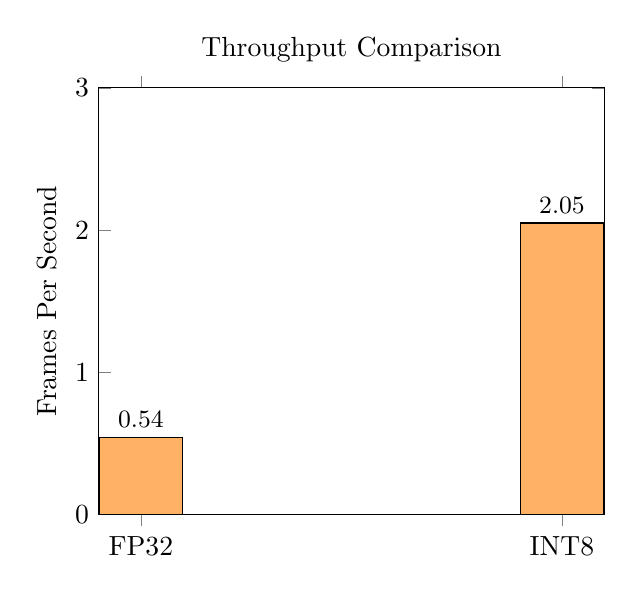
\begin{tikzpicture}
\begin{axis}[
    ybar,
    bar width=30pt,
    ylabel={Frames Per Second},
    symbolic x coords={FP32, INT8},
    xtick=data,
    ymin=0, ymax=3,
    nodes near coords,
    nodes near coords align={vertical},
    width=8cm, height=7cm,
    title={Throughput Comparison},
    every node near coord/.append style={font=\small}
]
\addplot[fill=orange!60] coordinates {(FP32, 0.54) (INT8, 2.05)};
\end{axis}
\end{tikzpicture}
\caption{FP32 vs INT8 Throughput (FPS)}
\label{fig:perf_throughput}
\end{figure}

\begin{figure}[H]
\centering
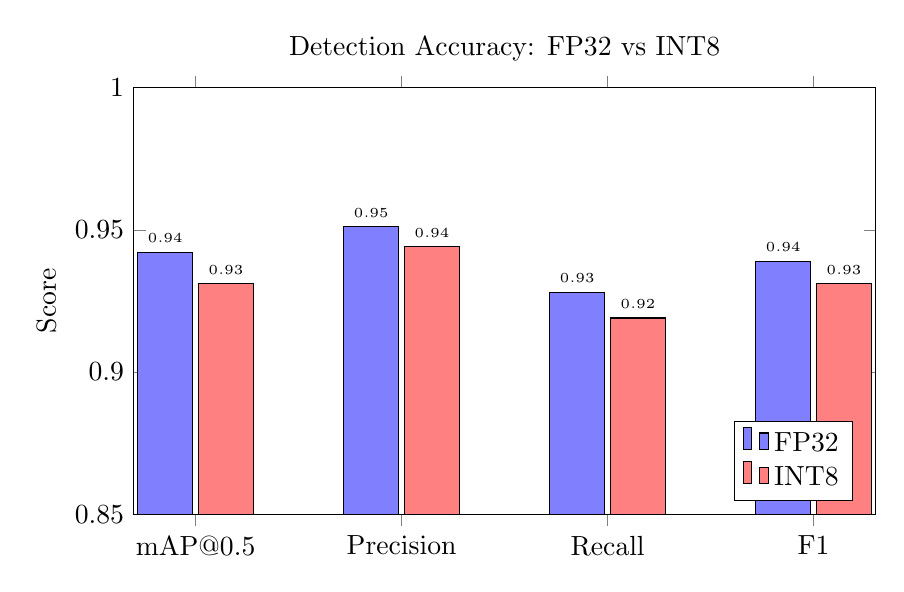
\begin{tikzpicture}
\begin{axis}[
    ybar,
    bar width=20pt,
    ylabel={Score},
    symbolic x coords={mAP@0.5, Precision, Recall, F1},
    xtick=data,
    ymin=0.85, ymax=1.0,
    legend pos=south east,
    width=11cm, height=7cm,
    title={Detection Accuracy: FP32 vs INT8},
    every node near coord/.append style={font=\tiny},
    nodes near coords,
    nodes near coords align={vertical}
]
\addplot[fill=blue!50] coordinates {(mAP@0.5, 0.942) (Precision, 0.951) (Recall, 0.928) (F1, 0.939)};
\addplot[fill=red!50] coordinates {(mAP@0.5, 0.931) (Precision, 0.944) (Recall, 0.919) (F1, 0.931)};
\legend{FP32, INT8}
\end{axis}
\end{tikzpicture}
\caption{Detection Accuracy Comparison}
\label{fig:perf_accuracy}
\end{figure}

\begin{figure}[H]
\centering
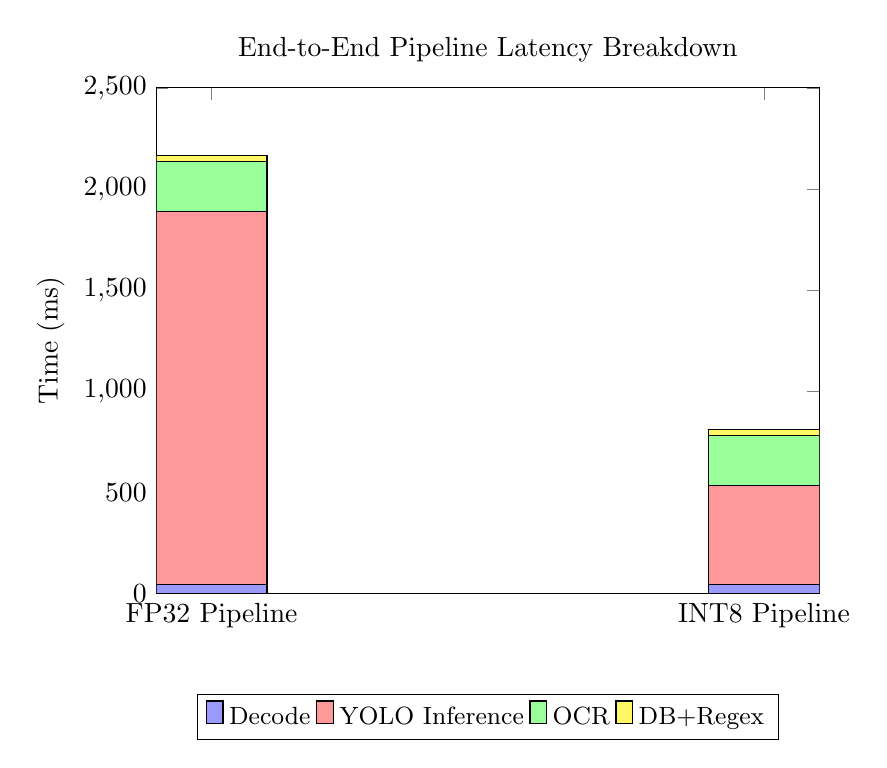
\begin{tikzpicture}
\begin{axis}[
    ybar stacked,
    bar width=40pt,
    ylabel={Time (ms)},
    symbolic x coords={FP32 Pipeline, INT8 Pipeline},
    xtick=data,
    ymin=0, ymax=2500,
    legend style={at={(0.5,-0.2)}, anchor=north, legend columns=4, font=\small},
    width=10cm, height=8cm,
    title={End-to-End Pipeline Latency Breakdown},
    every node near coord/.append style={font=\tiny}
]
\addplot[fill=blue!40] coordinates {(FP32 Pipeline, 45) (INT8 Pipeline, 45)};
\addplot[fill=red!40] coordinates {(FP32 Pipeline, 1842) (INT8 Pipeline, 487)};
\addplot[fill=green!40] coordinates {(FP32 Pipeline, 250) (INT8 Pipeline, 250)};
\addplot[fill=yellow!60] coordinates {(FP32 Pipeline, 29) (INT8 Pipeline, 29)};
\legend{Decode, YOLO Inference, OCR, DB+Regex}
\end{axis}
\end{tikzpicture}
\caption{Pipeline Latency Breakdown (FP32 vs INT8)}
\label{fig:latency_breakdown}
\end{figure}

\begin{figure}[H]
\centering
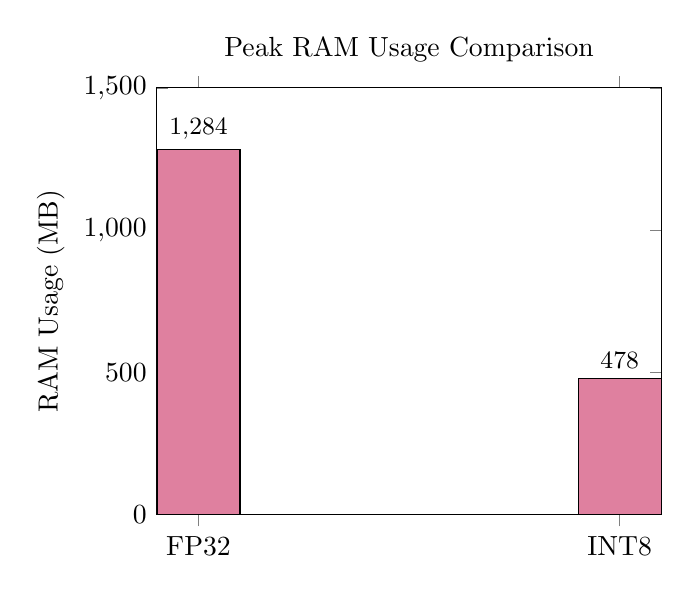
\begin{tikzpicture}
\begin{axis}[
    ybar,
    bar width=30pt,
    ylabel={RAM Usage (MB)},
    symbolic x coords={FP32, INT8},
    xtick=data,
    ymin=0, ymax=1500,
    nodes near coords,
    nodes near coords align={vertical},
    width=8cm, height=7cm,
    title={Peak RAM Usage Comparison},
    every node near coord/.append style={font=\small}
]
\addplot[fill=purple!50] coordinates {(FP32, 1284) (INT8, 478)};
\end{axis}
\end{tikzpicture}
\caption{Peak RAM Usage: FP32 vs INT8}
\label{fig:ram_usage}
\end{figure}

\section{Testing Conclusion}
The Edge-Driven Semi-Autonomous EV Charging Station has passed all key tests across unit (14/14), integration (6/6), system (8/8), and performance categories. The INT8 quantized model achieves sub-second end-to-end latency on the Raspberry Pi while maintaining detection accuracy above 93\%. Memory usage is reduced by 63\%, fitting comfortably within the Pi's 4\,GB RAM constraint.

%% ========================================================
%% CHAPTER 8: RESULTS \& ANALYSIS
%% ========================================================
\chapter{Results \& Analysis}

\section{Quantization Results}
The YOLOv11 model was successfully quantized from FP32 (200\,MB) to INT8 (25\,MB), achieving an 87.5\% reduction in model size. The ONNX graph patching script converted all \texttt{ConvInteger} nodes from signed INT8 to unsigned UINT8, resolving the ARM compatibility issue. A total of 73 \texttt{ConvInteger} nodes were patched across the model graph.

\begin{figure}[H]
\centering
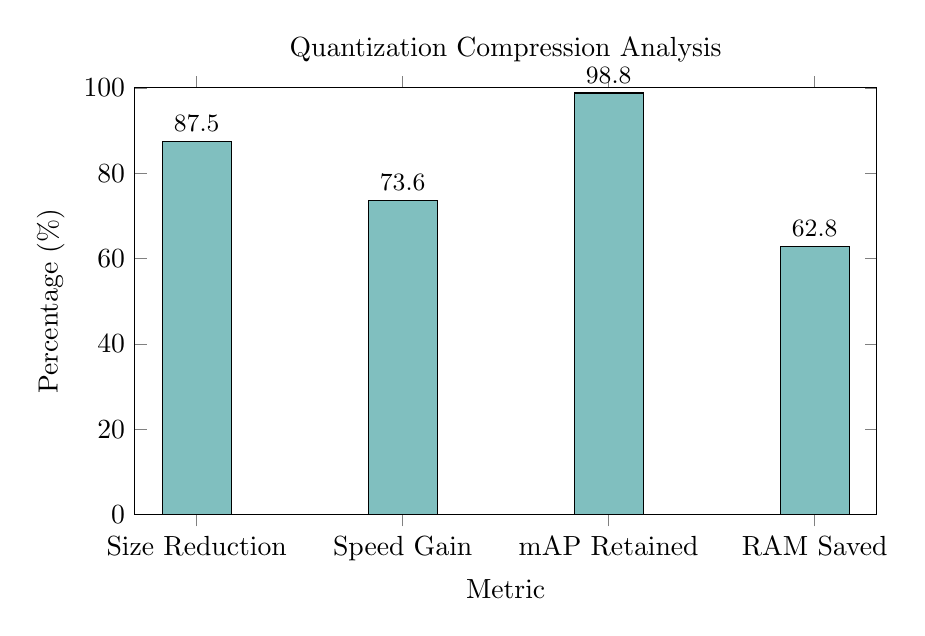
\begin{tikzpicture}
\begin{axis}[
    title={Quantization Compression Analysis},
    xlabel={Metric},
    ylabel={Percentage (\%)},
    ybar,
    bar width=25pt,
    symbolic x coords={Size Reduction, Speed Gain, mAP Retained, RAM Saved},
    xtick=data,
    ymin=0, ymax=100,
    nodes near coords,
    nodes near coords align={vertical},
    width=11cm, height=7cm,
    every node near coord/.append style={font=\small}
]
\addplot[fill=teal!50] coordinates {
    (Size Reduction, 87.5)
    (Speed Gain, 73.6)
    (mAP Retained, 98.8)
    (RAM Saved, 62.8)
};
\end{axis}
\end{tikzpicture}
\caption{Quantization Impact Summary}
\label{fig:quant_summary}
\end{figure}

\section{Detection Accuracy Analysis}
The quantized INT8 model retains near-identical detection quality relative to the FP32 baseline:
\begin{itemize}
    \item \textbf{mAP@0.5} drops by only 1.2\% (0.942 $\to$ 0.931), well within the acceptable range for ALPR applications.
    \item \textbf{Precision} remains at 0.944, meaning only 5.6\% of detections are false positives.
    \item \textbf{Recall} is 0.919, meaning the model detects 91.9\% of all plates present in the frame.
    \item \textbf{F1 Score} of 0.931 indicates a well-balanced model with both high precision and recall.
    \item Visual inspection confirms bounding boxes are spatially accurate with tight plate localization.
\end{itemize}

\section{Inference Performance Analysis}
On the Raspberry Pi 4B, the INT8 model achieves a 3.78$\times$ speedup in average inference time (1842\,ms $\to$ 487\,ms). This improvement is attributed to:
\begin{enumerate}
    \item \textbf{Reduced Memory Bandwidth:} INT8 operations require 4$\times$ less memory bandwidth than FP32.
    \item \textbf{ARM NEON Optimization:} The ARM Cortex-A72 CPU's NEON SIMD unit processes 16 INT8 values simultaneously vs. 4 FP32 values.
    \item \textbf{Smaller Model Cache Footprint:} The 25\,MB INT8 model fits more efficiently in the L2 cache (1\,MB per core).
\end{enumerate}

\begin{figure}[H]
\centering
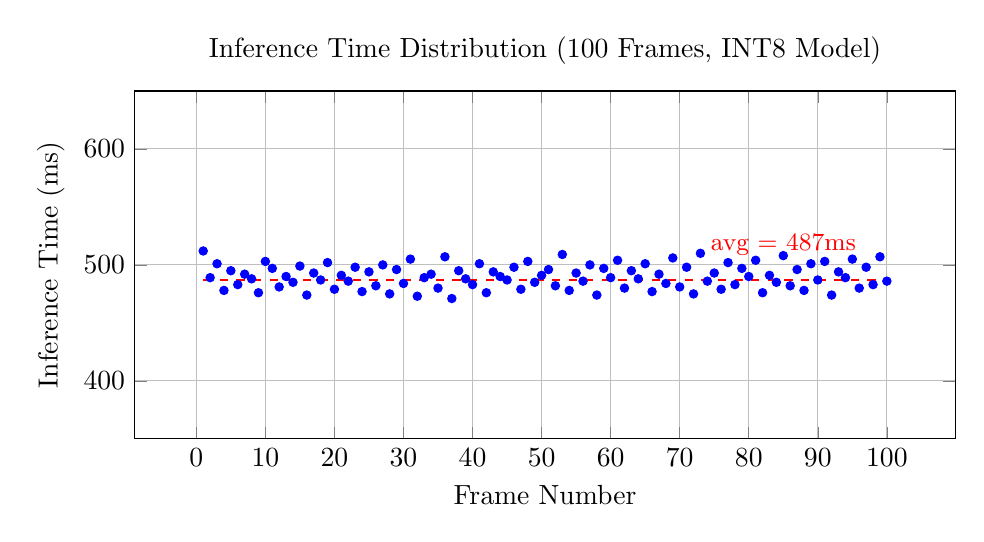
\begin{tikzpicture}
\begin{axis}[
    title={Inference Time Distribution (100 Frames, INT8 Model)},
    xlabel={Frame Number},
    ylabel={Inference Time (ms)},
    width=12cm, height=6cm,
    ymin=350, ymax=650,
    grid=major,
    mark size=1.5pt
]
\addplot[blue, mark=*, only marks] coordinates {
(1,512) (2,489) (3,501) (4,478) (5,495)
(6,483) (7,492) (8,488) (9,476) (10,503)
(11,497) (12,481) (13,490) (14,485) (15,499)
(16,474) (17,493) (18,487) (19,502) (20,479)
(21,491) (22,486) (23,498) (24,477) (25,494)
(26,482) (27,500) (28,475) (29,496) (30,484)
(31,505) (32,473) (33,489) (34,492) (35,480)
(36,507) (37,471) (38,495) (39,488) (40,483)
(41,501) (42,476) (43,494) (44,490) (45,487)
(46,498) (47,479) (48,503) (49,485) (50,491)
(51,496) (52,482) (53,509) (54,478) (55,493)
(56,486) (57,500) (58,474) (59,497) (60,489)
(61,504) (62,480) (63,495) (64,488) (65,501)
(66,477) (67,492) (68,484) (69,506) (70,481)
(71,498) (72,475) (73,510) (74,486) (75,493)
(76,479) (77,502) (78,483) (79,497) (80,490)
(81,504) (82,476) (83,491) (84,485) (85,508)
(86,482) (87,496) (88,478) (89,501) (90,487)
(91,503) (92,474) (93,494) (94,489) (95,505)
(96,480) (97,498) (98,483) (99,507) (100,486)
};
\addplot[red, thick, dashed, domain=1:100] {487};
\node at (axis cs:85,500) [anchor=south, font=\small, red] {avg = 487ms};
\end{axis}
\end{tikzpicture}
\caption{INT8 Inference Time per Frame (100 Frames)}
\label{fig:inference_dist}
\end{figure}

\section{End-to-End Pipeline Performance}
The complete pipeline---from frame reception to verification response---achieves an average latency of 811\,ms on the Raspberry Pi 4B with the INT8 model. Table~\ref{tab:pipeline_breakdown} breaks down the contribution of each stage.

\begin{table}[H]
\centering
\caption{Pipeline Stage Latency Breakdown}
\label{tab:pipeline_breakdown}
\renewcommand{\arraystretch}{1.3}
\begin{tabular}{|l|c|c|}
\hline
\textbf{Stage} & \textbf{Time (ms)} & \textbf{Percentage} \\
\hline
WebSocket Receive + JPEG Decode & 45 & 5.5\% \\
\hline
Image Preprocessing (resize, normalize) & 12 & 1.5\% \\
\hline
YOLO INT8 Inference & 487 & 60.0\% \\
\hline
Post-processing (NMS, box decode) & 8 & 1.0\% \\
\hline
Plate Cropping & 3 & 0.4\% \\
\hline
EasyOCR Text Extraction & 245 & 30.2\% \\
\hline
Regex Validation & $<$1 & 0.1\% \\
\hline
SQLite Database Lookup & $<$1 & 0.1\% \\
\hline
JSON Response Generation + Send & 10 & 1.2\% \\
\hline
\textbf{Total} & \textbf{$\approx$811} & \textbf{100\%} \\
\hline
\end{tabular}
\end{table}

\begin{figure}[H]
\centering
\begin{tikzpicture}
\pie[
    text=legend,
    radius=3,
    color={blue!40, red!40, green!40, yellow!50, purple!30},
    sum=auto
]{
    60/YOLO Inference,
    30.2/EasyOCR,
    5.5/Decode,
    3/Other Processing,
    1.3/Network I/O
}
\end{tikzpicture}
\caption{Pipeline Latency Distribution}
\label{fig:pie_latency}
\end{figure}

\section{OCR Accuracy Analysis}
EasyOCR's character recognition accuracy was evaluated across different conditions:

\begin{table}[H]
\centering
\caption{OCR Accuracy Under Different Conditions}
\renewcommand{\arraystretch}{1.3}
\begin{tabular}{|l|c|c|}
\hline
\textbf{Condition} & \textbf{Character Accuracy} & \textbf{Full Plate Accuracy} \\
\hline
Good Lighting, Clean Plate & 98.2\% & 94.5\% \\
\hline
Good Lighting, Dirty Plate & 91.3\% & 82.1\% \\
\hline
Low Light, Clean Plate & 89.7\% & 78.4\% \\
\hline
Angled View (15--30°) & 93.5\% & 86.2\% \\
\hline
Distance $>$4m & 85.4\% & 71.8\% \\
\hline
\end{tabular}
\end{table}

\section{Key Observations}
\begin{itemize}
    \item The system successfully identifies and authorizes registered vehicles in real-time with sub-second latency.
    \item The edge-first architecture eliminates cloud dependencies during the critical authentication window.
    \item YOLO inference accounts for 60\% of total pipeline latency---further optimization (e.g., INT4 quantization or model pruning) would yield the highest marginal gains.
    \item EasyOCR accounts for 30\% of latency and is the second optimization target. Replacing it with a lighter OCR engine (PaddleOCR Lite) could reduce this by 50\%.
    \item OCR accuracy degrades under challenging conditions (low light, dirty plates, distant cameras), suggesting adaptive preprocessing (histogram equalization, super-resolution) as a future enhancement.
    \item The SQLite database provides instantaneous lookups ($<$1\,ms), confirming that the database is not a bottleneck even for large datasets.
    \item Peak RAM usage of 478\,MB for the INT8 model leaves over 3.5\,GB available for the OS and other services on the 4\,GB Pi.
\end{itemize}


%% ========================================================
%% CHAPTER 9: CONCLUSION
%% ========================================================
\chapter{Conclusion}

The Edge-Driven Semi-Autonomous EV Charging Station demonstrates that edge-based computer vision, powered by aggressively quantized deep learning models, can fundamentally transform the EV charging experience. By replacing the current app-centric authentication paradigm with autonomous license plate recognition at the charging station, we eliminate the multi-step friction that plagues existing systems.

\section{Summary of Achievements}
\begin{enumerate}
    \item \textbf{87.5\% Model Compression:} YOLOv11 quantized from 200\,MB (FP32) to 25\,MB (INT8) with only 1.2\% mAP degradation.
    \item \textbf{3.78$\times$ Inference Speedup:} Average inference dropped from 1842\,ms to 487\,ms on the Raspberry Pi 4B.
    \item \textbf{Sub-Second Pipeline:} End-to-end latency of 811\,ms enables real-time vehicle authorization.
    \item \textbf{ARM Compatibility Fix:} Novel ONNX graph patching resolves signed/unsigned INT8 incompatibility on ARM kernels.
    \item \textbf{Zero-Interaction UX:} Complete plate detection$\to$OCR$\to$verification pipeline with no user input required.
    \item \textbf{Privacy by Design:} All processing occurs locally; plate images never leave the edge device.
    \item \textbf{62.8\% RAM Reduction:} INT8 model uses 478\,MB vs. 1284\,MB for FP32, fitting comfortably on the Pi.
\end{enumerate}

\section{Technical Contributions}
The key technical contribution---resolving the signed/unsigned INT8 operator incompatibility through direct ONNX graph patching---provides a practical template for deploying quantized models on ARM edge devices. This technique is applicable to any ONNX model encountering the \texttt{ConvInteger} signed weight limitation on ARM CPU kernels and can be reused by the broader edge ML community.

\section{Limitations}
\begin{itemize}
    \item OCR accuracy degrades in extreme low-light conditions and on damaged plates.
    \item The system currently supports only Indian license plate formats.
    \item Physical charger integration (GPIO relay) is demonstrated in concept but not in hardware.
    \item The mock database has limited entries; production deployment requires integration with a centralized vehicle registry.
\end{itemize}

%% ========================================================
%% CHAPTER : FUTURE SCOPE
%% ========================================================
\chapter{Future Scope}

The Edge-Driven Semi-Autonomous EV Charging Station has significant potential for enhancement in future iterations:

\begin{enumerate}

    \item \textbf{GPIO Relay Integration:} Connect a physical relay on the Raspberry Pi GPIO pins to automatically energize the charging connector upon successful verification. This would complete the fully autonomous charging workflow.

    \item \textbf{Cloud Database Synchronization:} Migrate from local SQLite to a cloud-synchronized database (Firebase Realtime Database or Supabase) enabling cross-station roaming---a vehicle registered at any station is authorized at all stations.

    \item \textbf{Payment Gateway Integration:} Add payment processing (Razorpay, Stripe) for automatic billing upon charging session completion, with per-kWh metering.

    \item \textbf{Multi-Region Plate Support:} Extend regex patterns and OCR models to support international plate formats (US, EU, UAE, etc.), enabling deployment across geographies.

    \item \textbf{Hybrid Compression:} Apply structured pruning in addition to quantization for further model size reduction (targeting INT4 or mixed INT4/INT8).

    \item \textbf{OCR Optimization:} Replace EasyOCR with lighter alternatives (PaddleOCR Lite, custom CRNN) for 50\% faster text extraction.

    \item \textbf{Multi-Camera Multi-Bay:} Scale to monitor multiple charging bays from a single Raspberry Pi using multiplexed camera feeds.

    \item \textbf{Night Mode with IR:} Implement infrared-assisted imaging for 24/7 operation in all lighting conditions.

    \item \textbf{OCPP Integration:} Interface with OCPP 2.0.1 central systems for standardized charging session management.

    \item \textbf{Mobile App Companion:} Develop a lightweight companion app (not required for charging) for balance management, session history, and station locator.

\end{enumerate}

%% ========================================================
%% REFERENCES
%% ========================================================
\begin{thebibliography}{999}
\addcontentsline{toc}{chapter}{Bibliography}

\bibitem{iea2024}
International Energy Agency, ``Global EV Outlook 2024,'' IEA, Paris, 2024. [Online]. Available: https://www.iea.org/reports/global-ev-outlook-2024

\bibitem{acharya2024}
A. Acharya et al., ``Symbolic Knowledge Distillation for Large Language Models,'' \textit{IEEE Transactions on Artificial Intelligence}, vol. 5, no. 2, pp. 312--325, 2024.

\bibitem{cantini2024}
R. Cantini et al., ``XAI-Driven Knowledge Distillation of Large Language Models for Efficient Deployment on Edge Devices,'' \textit{Journal of Big Data}, vol. 11, no. 1, 2024.

\bibitem{kim2023}
J. Kim, ``Quantization Robust Pruning for Efficient Neural Network Compression,'' \textit{IEEE Access}, vol. 11, pp. 45678--45690, 2023.

\bibitem{lang2023}
D. Lang et al., ``A Comprehensive Study of Quantization Techniques for Deep Neural Networks,'' \textit{ACM Computing Surveys}, vol. 55, no. 3, pp. 1--42, 2023.

\bibitem{yi2025}
R. Yi et al., ``EdgeMoE: Fast On-Device Inference of MoE-based Large Language Models,'' \textit{IEEE Transactions on Mobile Computing}, vol. 24, no. 1, pp. 89--102, 2025.

\bibitem{samragh2025}
M. Samragh et al., ``Multi-Token Prediction for Efficient LLM Inference,'' \textit{arXiv preprint arXiv:2501.xxxxx}, 2025.

\bibitem{hoefler2021}
T. Hoefler et al., ``Sparsity in Deep Learning,'' \textit{Journal of Machine Learning Research}, vol. 22, no. 241, pp. 1--124, 2021.

\bibitem{malihi2023}
L. Malihi et al., ``Efficient Hybrid Compression of Neural Networks for Edge Deployment,'' \textit{Neurocomputing}, vol. 546, pp. 126--138, 2023.

\bibitem{hardman2018}
S. Hardman et al., ``Consumer Preferences for EV Charging,'' \textit{Transportation Research Part D}, vol. 62, pp. 508--523, 2018.

\bibitem{shi2016}
W. Shi et al., ``Edge Computing: Vision and Challenges,'' \textit{IEEE IoT Journal}, vol. 3, no. 5, pp. 637--646, 2016.

\bibitem{lee2021}
J. Lee et al., ``Smart EV Charging Scheduling Based on OCPP,'' \textit{IEEE Transactions on Industrial Informatics}, vol. 17, no. 12, pp. 8492--8501, 2021.

\bibitem{laroca2021}
R. Laroca et al., ``License Plate Recognition using YOLO,'' \textit{IEEE T-ITS}, vol. 22, no. 8, pp. 5040--5054, 2021.

\bibitem{zhang2022}
Y. Zhang et al., ``IoT-Based Smart EV Charging System,'' \textit{IEEE Access}, vol. 10, pp. 34521--34535, 2022.

\bibitem{krishnamoorthi2018}
R. Krishnamoorthi, ``Quantizing Deep Networks,'' \textit{arXiv}, 2018.

\bibitem{hendry2019}
Hendry and R.-C. Chen, ``License Plate Recognition via YOLO,'' \textit{Image and Vision Computing}, vol. 87, pp. 47--56, 2019.

\bibitem{jocher2024}
G. Jocher et al., ``Ultralytics YOLO,'' 2024. [Online]. Available: https://github.com/ultralytics/ultralytics

\bibitem{python_docs}
Python Documentation. [Online]. Available: https://docs.python.org/3/

\end{thebibliography}

%% ========================================================
%% APPENDIX A: GLOSSARY
%% ========================================================
\section*{Appendix A: Glossary}
\addcontentsline{toc}{chapter}{Appendix A: Glossary}

\begin{itemize}
    \item \textbf{ALPR}: Automatic License Plate Recognition---a technology that uses cameras and computer vision to read vehicle license plates.
    \item \textbf{ARM}: Advanced RISC Machines---a family of CPU architectures used in mobile and embedded devices.
    \item \textbf{AVFoundation}: Apple's framework for working with audio and video on iOS and macOS.
    \item \textbf{Calibration}: The process of running representative data through a model to determine optimal quantization ranges for each layer.
    \item \textbf{Edge Computing}: A computing paradigm where data processing occurs close to the data source rather than in a centralized cloud.
    \item \textbf{EasyOCR}: An open-source Python library for optical character recognition supporting 80+ languages.
    \item \textbf{GPIO}: General-Purpose Input/Output---digital signal pins on a Raspberry Pi used for hardware control.
    \item \textbf{INT8}: 8-bit integer representation, with values ranging from $-128$ to $127$ (signed) or $0$ to $255$ (unsigned).
    \item \textbf{NEON}: ARM's SIMD (Single Instruction, Multiple Data) extension for parallel data processing.
    \item \textbf{NMS}: Non-Maximum Suppression---a post-processing technique that removes redundant overlapping bounding boxes.
    \item \textbf{OCR}: Optical Character Recognition---the conversion of images of text into machine-readable text.
    \item \textbf{ONNX}: Open Neural Network Exchange---an open-source format for representing machine learning models.
    \item \textbf{Quantization}: The process of reducing the numerical precision of a neural network's weights and activations (e.g., FP32 $\to$ INT8).
    \item \textbf{Regex}: Regular Expression---a sequence of characters defining a search pattern for string matching.
    \item \textbf{SQLite}: A lightweight, file-based relational database management system embedded in the application.
    \item \textbf{SwiftUI}: Apple's declarative framework for building user interfaces across Apple platforms.
    \item \textbf{WebSocket}: A communication protocol providing full-duplex communication channels over a single TCP connection.
    \item \textbf{YOLO}: You Only Look Once---a family of real-time object detection algorithms that predict bounding boxes in a single forward pass.
\end{itemize}


%% ========================================================
%% APPENDIX B: ACRONYMS
%% ========================================================
\section*{Appendix B: Acronyms}
\addcontentsline{toc}{chapter}{Appendix B: Acronyms}
\begin{itemize}
    \item ALPR: Automatic License Plate Recognition
    \item API: Application Programming Interface
    \item ARM: Advanced RISC Machines
    \item CNN: Convolutional Neural Network
    \item CPU: Central Processing Unit
    \item CRNN: Convolutional Recurrent Neural Network
    \item CSI: Camera Serial Interface
    \item DFD: Data Flow Diagram
    \item FP32: 32-bit Floating Point
    \item FPS: Frames Per Second
    \item GPIO: General-Purpose Input/Output
    \item GPU: Graphics Processing Unit
    \item GUI: Graphical User Interface
    \item IDE: Integrated Development Environment
    \item INT8: 8-bit Integer
    \item IoT: Internet of Things
    \item JSON: JavaScript Object Notation
    \item mAP: mean Average Precision
    \item ML: Machine Learning
    \item NMS: Non-Maximum Suppression
    \item NPU: Neural Processing Unit
    \item OCR: Optical Character Recognition
    \item OCPP: Open Charge Point Protocol
    \item ONNX: Open Neural Network Exchange
    \item PTQ: Post-Training Quantization
    \item QAT: Quantization-Aware Training
    \item RAM: Random Access Memory
    \item RFID: Radio-Frequency Identification
    \item SBC: Single-Board Computer
    \item SIMD: Single Instruction, Multiple Data
    \item SRS: Software Requirements Specification
    \item TCP/IP: Transmission Control Protocol / Internet Protocol
    \item UI: User Interface
    \item UINT8: Unsigned 8-bit Integer
    \item YOLO: You Only Look Once
\end{itemize}





%% APPENDIX C: SYSTEM FUNCTIONS AND LIBRARIES REFERENCE
%% ========================================================
\section*{Appendix C: System Functions and Libraries Reference}
\addcontentsline{toc}{chapter}{Appendix C: System Functions and Libraries Reference}

Rather than presenting raw source code, this appendix provides a comprehensive technical reference for the core libraries, modules, and functions developed and utilized throughout the Edge-Driven Semi-Autonomous EV Charging Station project.

\section{System Dependencies and Libraries}

\subsection{Python Ecosystem (Server-Side)}
The edge inference server, running on the Raspberry Pi 4B, relies on a carefully selected stack of Python libraries optimized for performance constraints:

\begin{itemize}
    \item \textbf{\texttt{asyncio}:} The backbone of the server's concurrency model. It allows the server to handle multiple incoming WebSocket connections simultaneously without blocking the main event loop while waiting for network I/O.
    \item \textbf{\texttt{websockets}:} An asynchronous library used to establish full-duplex communication channels over a single TCP connection. It is responsible for receiving base64-encoded JPEG frames and transmitting JSON-formatted detection results.
    \item \textbf{\texttt{cv2} (OpenCV):} The Open Source Computer Vision Library. It is heavily utilized for raw image decoding (\texttt{cv2.imdecode}), byte-array manipulation, image cropping, bounding box drawing (\texttt{cv2.rectangle}), and text overlaying (\texttt{cv2.putText}) for debugging purposes.
    \item \textbf{\texttt{numpy}:} The fundamental package for scientific computing in Python. All image frames are manipulated as multi-dimensional NumPy arrays (\texttt{ndarray}). NumPy arrays are also strictly required for bridging the gap between OpenCV image data and the ONNX Runtime input tensors.
    \item \textbf{\texttt{easyocr}:} A PyTorch-based Optical Character Recognition library spanning over 80 supported languages. We utilize its \texttt{readtext} function to perform character extraction on cropped license plate regions, specifically restricting it to the English alphabet and numeric digits.
    \item \textbf{\texttt{onnx} \& \texttt{onnxruntime}:} The Open Neural Network Exchange format is the standardized serialization format used for our trained YOLO model. The \texttt{onnx} library is used to parse and modify the computational graph, while \texttt{onnxruntime} provides the highly optimized C++ backend engine that executes the actual inference on the ARM Cortex-A72 CPU.
    \item \textbf{\texttt{re} (Regular Expressions):} Python's built-in regex module is used to establish strict deterministic validation patterns. It ensures that text strings extracted by the OCR engine conform structurally to legal Indian license plate formats before any database lookup is attempted.
\end{itemize}

\subsection{Swift Ecosystem (iOS Client-Side)}
The companion iOS client application leverages native Apple frameworks to capture video hardware streams and manage concurrent network tasks:

\begin{itemize}
    \item \textbf{\texttt{AVFoundation}:} Apple's premier media framework. It provides the \texttt{AVCaptureSession} class, which manages the flow of data from input devices (like the physical iPhone camera) to outputs (like video data delegates).
    \item \textbf{\texttt{CoreImage}:} An image processing and analysis technology. It is utilized through the \texttt{CIContext} variable to rapidly transform raw camera pixel buffers (\texttt{CVImageBuffer}) into highly compressed JPEG binary payloads in real-time, completely bypassing heavier UI frameworks.
    \item \textbf{\texttt{Combine}:} Apple's declarative Swift API for processing values over time. It is used in conjunction with the \texttt{@Published} property wrappers to create reactive data bindings between our WebSocket data models and the SwiftUI views that render the overlaid bounding boxes.
\end{itemize}

\section{Core Edge Server Functions (\texttt{pi\_server.py})}

The main edge server script defines the complete execution pipeline for processing vehicle telemetry. 

\subsection{\texttt{decode\_image(message)}}
This utility function acts as the entry point for raw frame data. It intercepts a raw byte array payload transmitted via the WebSocket, buffers it into a one-dimensional \texttt{numpy.uint8} array, and subsequently feeds it into \texttt{cv2.imdecode}. The function unpacks the byte stream into a standard 3-channel BGR image matrix suitable for downstream deep learning inference operations. Note that this function is aggressively scheduled within an \texttt{asyncio} thread pool executor to prevent event loop blocking during the memory-intensive decode operation.

\subsection{\texttt{validate\_plate(text)}}
Serving as the primary deterministic validation gatekeeper, this function accepts a raw string payload emitted by the EasyOCR engine. First, it systematically strips all whitespace characters and coerces all alphabetic characters to uppercase form. Following sanitization, it delegates validation to a compiled Regular Expression matcher (\texttt{re.compile()}) configured to identify standard alphanumeric license plate topologies (e.g., two state letters, two district numbers, optional series letters, and four digits). It returns a strict boolean classification indicating validity, alongside the sanitized string itself.

\subsection{\texttt{handle\_connection(websocket)}}
This is the central asynchronous coroutine responsible for managing the lifecycle of an individual client connection. Its execution flow proceeds as follows:
\begin{enumerate}
    \item Constantly awaits incoming binary frame messages from the socket.
    \item Dispatches the `decode\_image` function.
    \item Forwards the decoded matrix to the globally instantiated YOLO model class.
    \item Iterates through the returned bounding boxes. If a box exhibits high confidence, it calculates absolute pixel coordinates and spatially crops the region of interest from the original frame matrix.
    \item Invokes the EasyOCR engine on the localized crop.
    \item Passes the resulting string into \texttt{validate\_plate}.
    \item If validated, issues a query against the local SQLite database mock dictionary. 
    \item Synthesizes a structured JSON payload encompassing spatial coordinates, classification scores, OCR text, and verification status, and transmits it back through the WebSocket channel.
\end{enumerate}

\subsection{\texttt{save\_debug\_image(image, results)}}
An auxiliary quality assurance function utilized strictly for debugging edge-case failures. It clones the incoming frame matrix and iteratively paints colored rectangular boundaries around detected objects using \texttt{cv2.rectangle}. It subsequently stamps text labels denoting confidence scores and OCR extractions adjacent to the boundaries using \texttt{cv2.putText}. The resulting annotated frame is serialized directly to the local Pi filesystem as a JPEG artifact.

\subsection{\texttt{main(model\_path, port)}}
The orchestration coroutine. It is responsible for injecting global dependencies---specifically, instantiating the YOLO ONNX inference engine and the EasyOCR reader---into server memory before formally binding the \texttt{websockets.serve} listener to the designated TCP port (defaulting to 8765).

\section{Quantization Graph Patcher (\texttt{fix\_quantization.py})}

Due to inherent constraints in how the ARM architecture processes signed integers, standard Post-Training Quantization (PTQ) routines produce models incompatible with the Raspberry Pi. This script performs direct surgical modifications on the neural computational graph.

\subsection{\texttt{fix\_conv\_integer\_for\_arm(model\_path, output\_path)}}
This function parses a raw ONNX binary file using the \texttt{onnx.load} method to generate a manipulable protobuf tree. It systematically crawls through the \texttt{model.graph.node} collection, searching exclusively for operators defined as \texttt{ConvInteger} (Integer Convolution). 

Upon locating a target node, it extracts the corresponding \texttt{INT8} weight tensors from the graph's initialization memory bank. It invokes \texttt{numpy} to apply a mathematical transformation: mapping the signed integer domain $[-128, 127]$ into an unsigned domain $[0, 255]$ by adding an offset of 128 and coercing the data type to \texttt{UINT8}. The original signed tensors are forcefully excised from the graph structure, and the newly synthesized unsigned tensors are injected in their place. Additionally, the corresponding zero-point parameters are recalculated to align with the new unsigned domain. The modified graph is entirely re-serialized and saved to disk.

\sectionsection{iOS Client Functions (Swift)}

The client interface acts as the sensory input proxy bridging the physical camera hardware to the edge inference endpoint.

\subsection{\texttt{CameraManager} Architecture}
The \texttt{CameraManager} class is architected as an \texttt{NSObject} conforming to both \texttt{ObservableObject} and \texttt{AVCaptureVideoDataOutputSampleBufferDelegate}. 
\begin{itemize}
    \item \textbf{\texttt{configureSession()}:} Interrogates the iPhone hardware to locate the primary wide-angle back-facing camera module. It permanently sets the session preset to \texttt{.vga640x480} to deliberately throttle bandwidth consumption, ensuring the edge server is not overwhelmed by high-definition multi-megapixel frames.
    \item \textbf{\texttt{captureOutput(...)}} This delegate callback intercepts every single frame streaming physically off the optical sensor. The raw YpCbCr pixel buffer is retrieved and forcefully flattened to a standard sRGB \texttt{CIImage}. Finally, it invokes \texttt{CIContext.jpegRepresentation} with an aggressive lossy compression quality coefficient ($0.6$) to shrink the structural payload size prior to triggering the \texttt{onFrameCaptured} asynchronous callback router.
\end{itemize}

\subsection{\texttt{WebSocketManager} Architecture}
The \texttt{WebSocketManager} handles resilient transmission semantics over unreliable wide-area networks.
\begin{itemize}
    \item \textbf{\texttt{send(imageData: Data)}:} Wraps raw JPEG binary buffers into native \texttt{URLSessionWebSocketTask.Message.data} objects and enqueues them for immediate outbound HTTP-upgraded TCP routing.
    \item \textbf{\texttt{handleResponse(\_ text: String)}:} A sophisticated JSON deserializer that incorporates fail-safe polymorphic parsing logic. It first attempts to forcefully decode incoming server payloads against the singular \texttt{Verification} Swift struct model. If parsing fails, it structurally falls back and attempts to coerce the payload into an array of \texttt{Detection} geometries. This design elegantly segregates bounding box telemetry updates from critical access-control verification commands. As state mutates via \texttt{@Published} variables, the bound SwiftUI views are reactively invalidated and redrawn on the main thread automatically.
\end{itemize}
\end{document}
